\section{系统架构}

\begin{figure}[t]
    \centerline{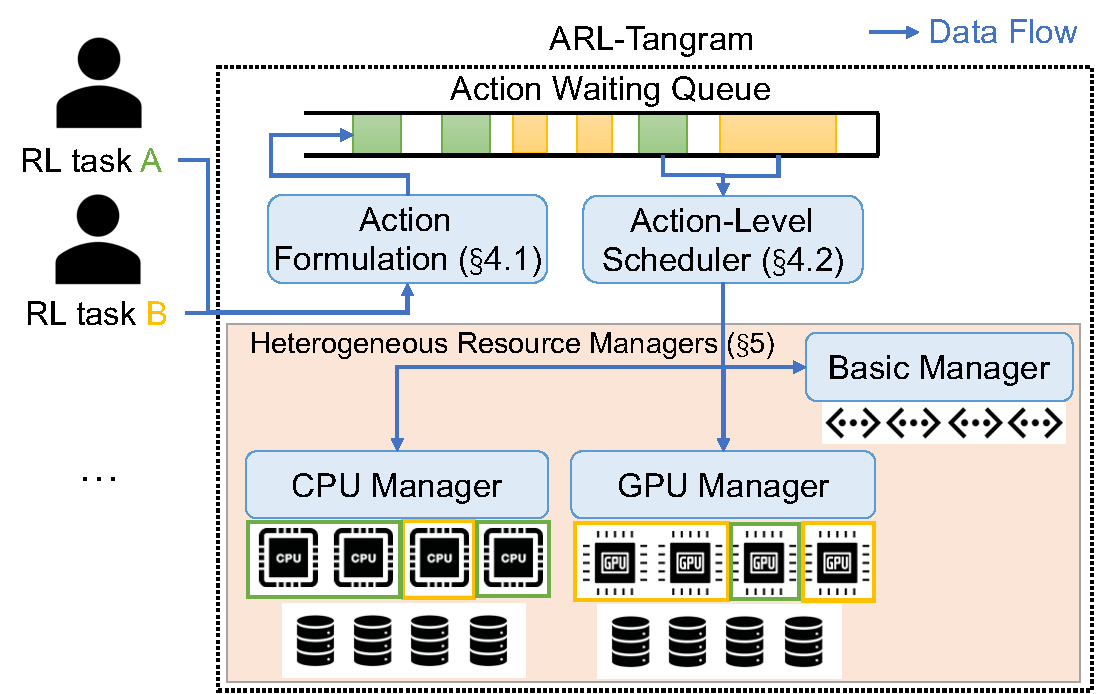
\includegraphics[width=0.6\linewidth]{figures/arch.pdf}}
    \vspace{-0.1in}
    \caption{\sysname 的系统总览。}
    \label{fig:arch_arch}
    \vspace{-0.15in}
\end{figure}

为了应对当前智能体 RL 训练中多层次的过量预留问题，无论是轨迹内部还是 RL 任务之间，我们提出了统一的动作级平台 \sysname。该架构将外部资源管理从主 RL 训练集群中解耦出来，把控制粒度从寿命较长的轨迹下沉到单个原子交互，也就是动作。

如图~\ref{fig:arch_arch} 所示，系统位于多种 RL 任务与异构外部资源之间，充当统一中介。其工作流程遵循标准化执行周期：(1) 动作提交：在 rollout 阶段，当智能体 LLM 调用工具或触发依赖外部资源的奖励计算时，它会向 \sysname 提交请求。(2) 统一建模与排队：\sysname 把不同的外部资源调用翻译成统一动作，并提交到统一动作队列。(3) 弹性调度：调度器在外部资源约束下调度等待队列中的动作，并与专门的资源管理器（如 CPU、GPU、API）协同，根据实时系统状态和动作建模结果进行弹性资源分配。(4) 动作执行：确定资源单位后，动作会在异构资源管理器分配到的资源上独立执行。(5) 结果回传与观测：动作执行完成后，结果会被传回 RL 框架，使其继续进行下一步 LLM 生成。

\sysname 主要包含三大组件，即动作建模模块（\S\ref{sec:design_modeling}）、动作级调度器（\S\ref{sec:design_scheduling}）和异构资源管理器（\S\ref{sec:design_resource_managing}）。这套架构的基础思想是把每一次原子调用都视作一个动作。因此，建模模块以统一方式刻画各种动作的成本和性能弹性；调度器则在资源约束下判断动作能否被调度，并以最小化动作完成时间（ACT）为目标为其弹性分配资源。这样，\sysname 能减少 LLM 等待外部资源返回的时间，进一步加速 RL 训练。获得调度决策后，异构资源管理器负责高效地分配与共享资源。借助统一资源接口，包括 Basic Manager、CPU Manager 和 GPU Manager 在内的管理器使用各自领域特定的技术来提升系统鲁棒性、资源利用率和动作执行速度。
